\documentclass[12pt,a4paper]{article}
\usepackage[utf8]{inputenc}
\usepackage[english,russian]{babel}
\usepackage{amssymb,amsfonts,amsmath,cite,enumerate,float,indentfirst}
\usepackage{graphicx}
\graphicspath{{images/}}
\usepackage{geometry}
\usepackage{systeme}
\usepackage{hyperref}
\usepackage{url}
\hypersetup{
	colorlinks,
	citecolor=black,
	filecolor=black,
	linkcolor=black,
	urlcolor=black
}
\geometry{left=2cm}
\geometry{right=1.5cm}
\geometry{top=2cm}
\geometry{bottom=2cm}
\begin{document}
	\begin{titlepage}
		\begin{center}		
			\vfill	
			Санкт-Петербургский политехнический университет \\
			Петра Великого\\
			\vskip 1cm
			Институт прикладной математики и механики \\
			Кафедра «Прикладная математика»
			\vfill
			\textbf{Отчёт\\
			по лабораторной работе №1\\
			по дисциплине\\
			«Математическая статистика»\\}
			\vfill
		\end{center}
		\vfill
		\hfill
		\begin{minipage}{0.4\textwidth}
			Выполнил студент:\\
			Петрунин Григорий Дмитриевич\\
			группа: 3630102/70201\\
		\end{minipage}
		\vfill
		\hfill 
		\begin{minipage}{0.4\textwidth}
			Проверил:\\
			к.ф.-м.н., доцент\\
			Баженов Александр Николаевич\
		\end{minipage}
		\vfill

		
		\begin{center}
			Санкт-Петербург\\2020 г.
		\end{center}
	\end{titlepage}

	\tableofcontents
	\newpage
	\section{Постановка задачи}
	Даны следующие 5 распределений вероятности:
	\begin{itemize}
		\item Нормальное распределение $\displaystyle N(x, 0, 1)$
		\item Распределение Коши $\displaystyle C(x, 0, 1)$
		\item Распределение Лапласа $\displaystyle L(x, 0, \frac{1}{\sqrt{2}}$)
		\item Равномерное распределение $\displaystyle U(x, -\sqrt{3}, \sqrt{3})$
		\item Распределение Пуассона $\displaystyle P(k, 10)$
	\end{itemize}
	Необходимо сгенерировать массивы данных (выборки) объемом 10, 50 и 100 элементов для каждого из вышеуказанных распределений. Для каждой выборки построить на одном графике гистограмму и соответствующую теоретическую плотность распределения. Описать полученный результат.
	\section{Теория}
	Приведем используемые в работе формулы плотностей распределения вероятности:
	\begin{itemize}
		\item Нормальное распределение:
			\begin{equation}
				N(x, 0, 1) = \frac{1}{\sqrt{2\pi}}e^{-\frac{x^2}{2}}
			\end{equation}
		\item Распределение Коши:
			\begin{equation}
				C(x, 0, 1) = \frac{1}{\pi(x^2+1)}
			\end{equation}
		\item Распределение Лапласа:
			\begin{equation}
				L(x, 0, \frac{1}{\sqrt{2}}) = \frac{1}{\sqrt{2}}e^{-\sqrt{2}|x|}
			\end{equation}
		\item Равномерное распределение:
			\begin{equation}
				U(x, -\sqrt{3}, \sqrt{3}) = \systeme*{\frac{1}{2\sqrt{3}} \hskip 0.5cm \mbox{если } |x| <= \sqrt{3}, 0 \hskip 0.5cm \mbox{если }|x| > \sqrt{3}}
			\end{equation}
		\item Распределение Пуассона:
			\begin{equation}
				P(k, 10) = \frac{10^k}{k!}e^{-10}
			\end{equation}
	\end{itemize}
	\newpage
	\section{Реализация}
		Задача выполнена с помощью языка программирования Python 3.8.1 в среде разработки PyCharm Community Edition 2019. Для статистических вычислений (генерация выборки и построение функции распределения) использовалась open-source библиотека SciPy (модуль scipy.stats), для отрисовки графиков - библиотека Matplotlib для Python, для вспомогательных операций - расширение-библиотека NumPy, предоставляющая широкий набор математических операций. Ссылка на исходный код вынесена в приложениях.
	\section{Результаты}
	\subsection{Нормальное распределение}
		\begin{figure}[h]
			\centering
			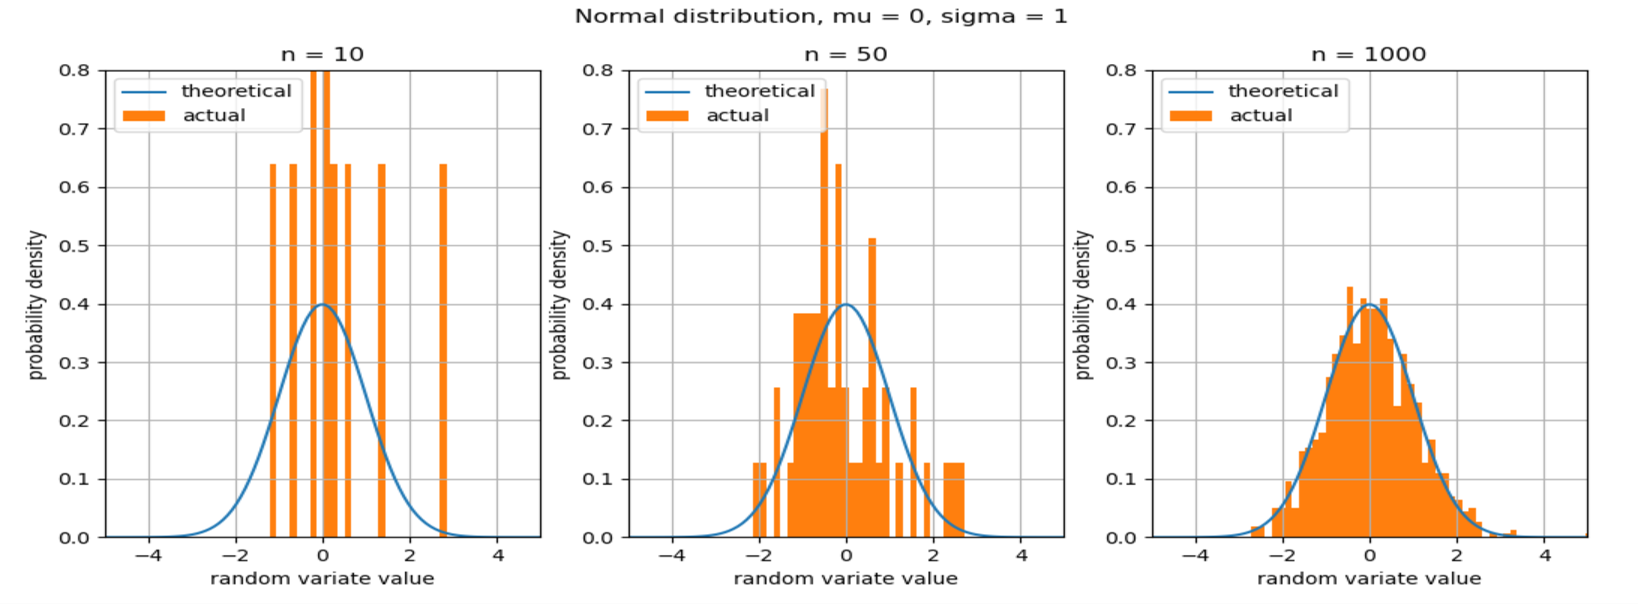
\includegraphics[width=\linewidth]{MS1res/normal.png}
			\caption{Графики нормального распределения и сгенерированной выборки}
		\end{figure}
	\subsection{Распределение Коши}
		\begin{figure}[h]
			\centering
			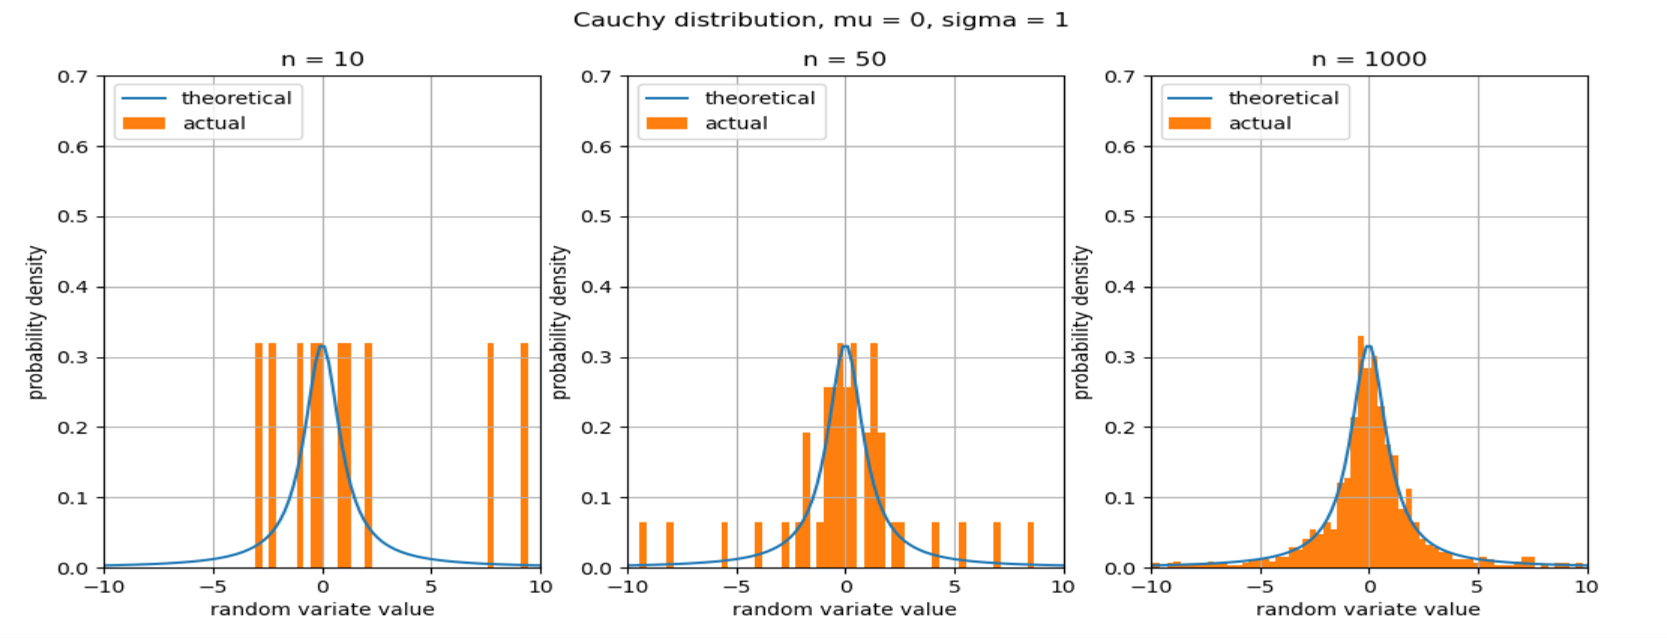
\includegraphics[width=\linewidth]{MS1res/cauchy.png}
			\caption{Графики распределения Коши и сгенерированной выборки}
		\end{figure}
	\subsection{Распределение Лапласа}
		\begin{figure}[h]
			\centering
			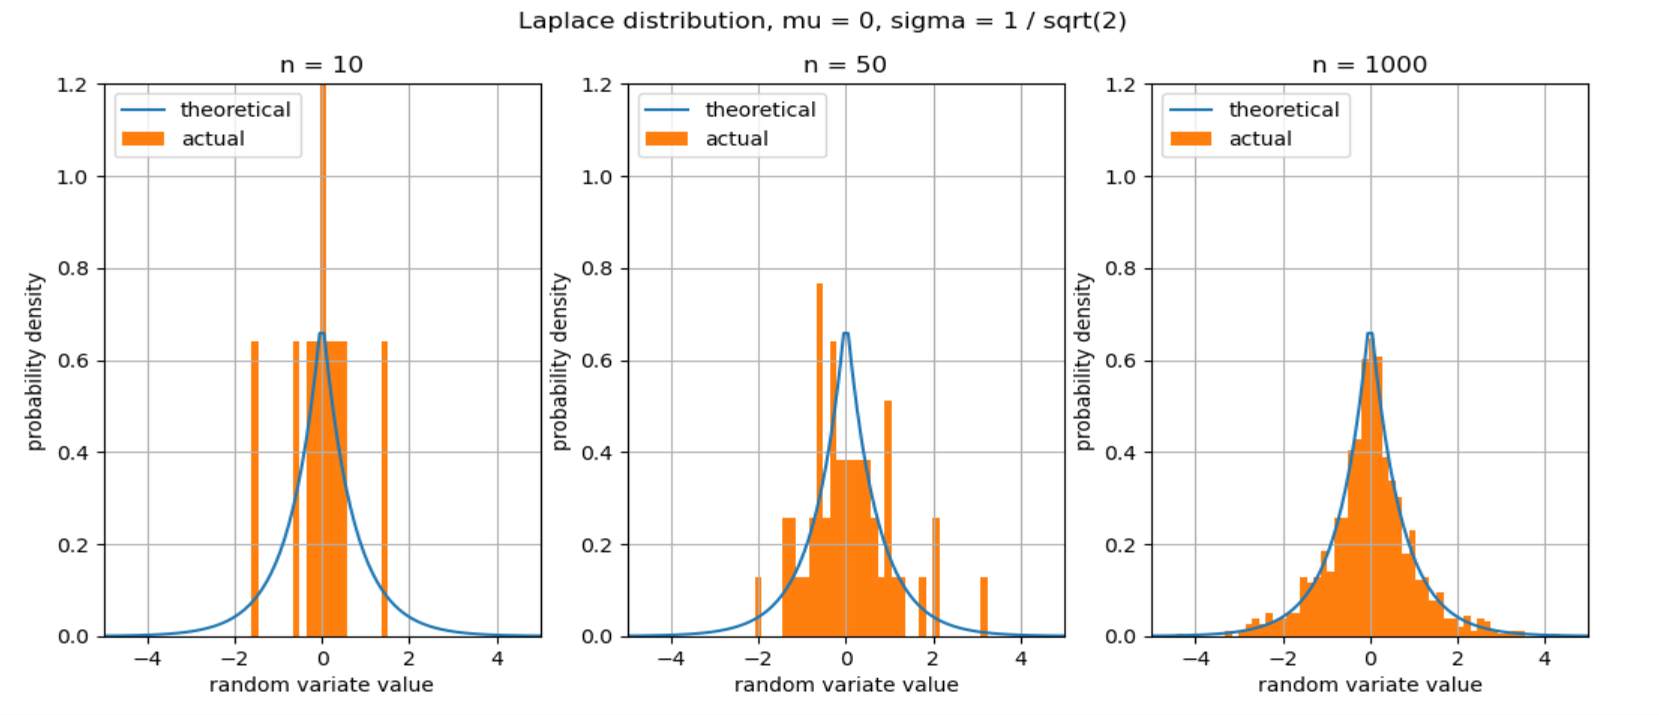
\includegraphics[width=\linewidth]{MS1res/laplace.png}
			\caption{Графики распределения Лапласа и сгенерированной выборки}
		\end{figure}
	\subsection{Равномерное распределение}
		\begin{figure}[h]
			\centering
			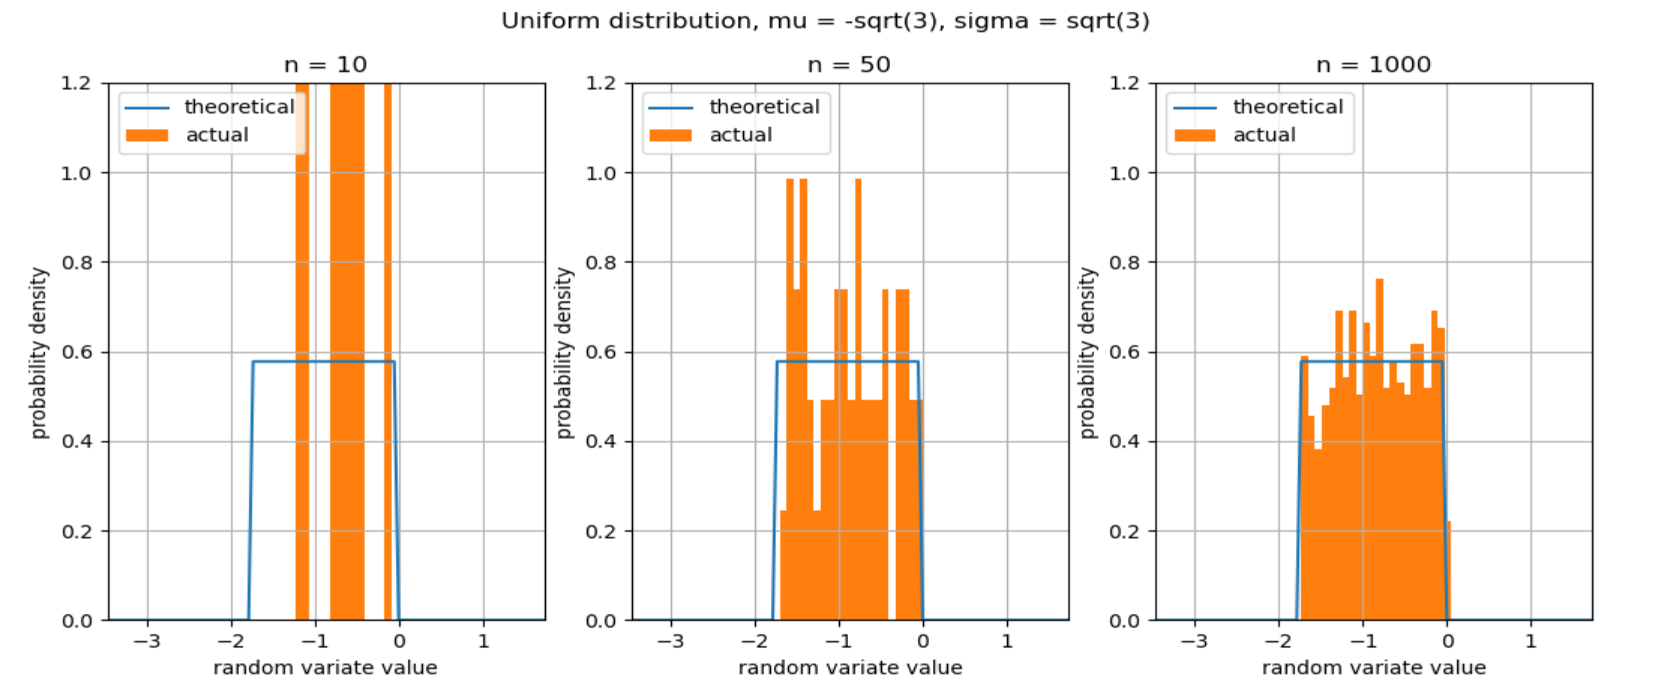
\includegraphics[width=\linewidth]{MS1res/uniform.png}
			\caption{Графики равномерного распределения и сгенерированной выборки}
		\end{figure}
	\newpage
	\subsection{Распределение Пуассона}
		\begin{figure}[h]
			\centering
			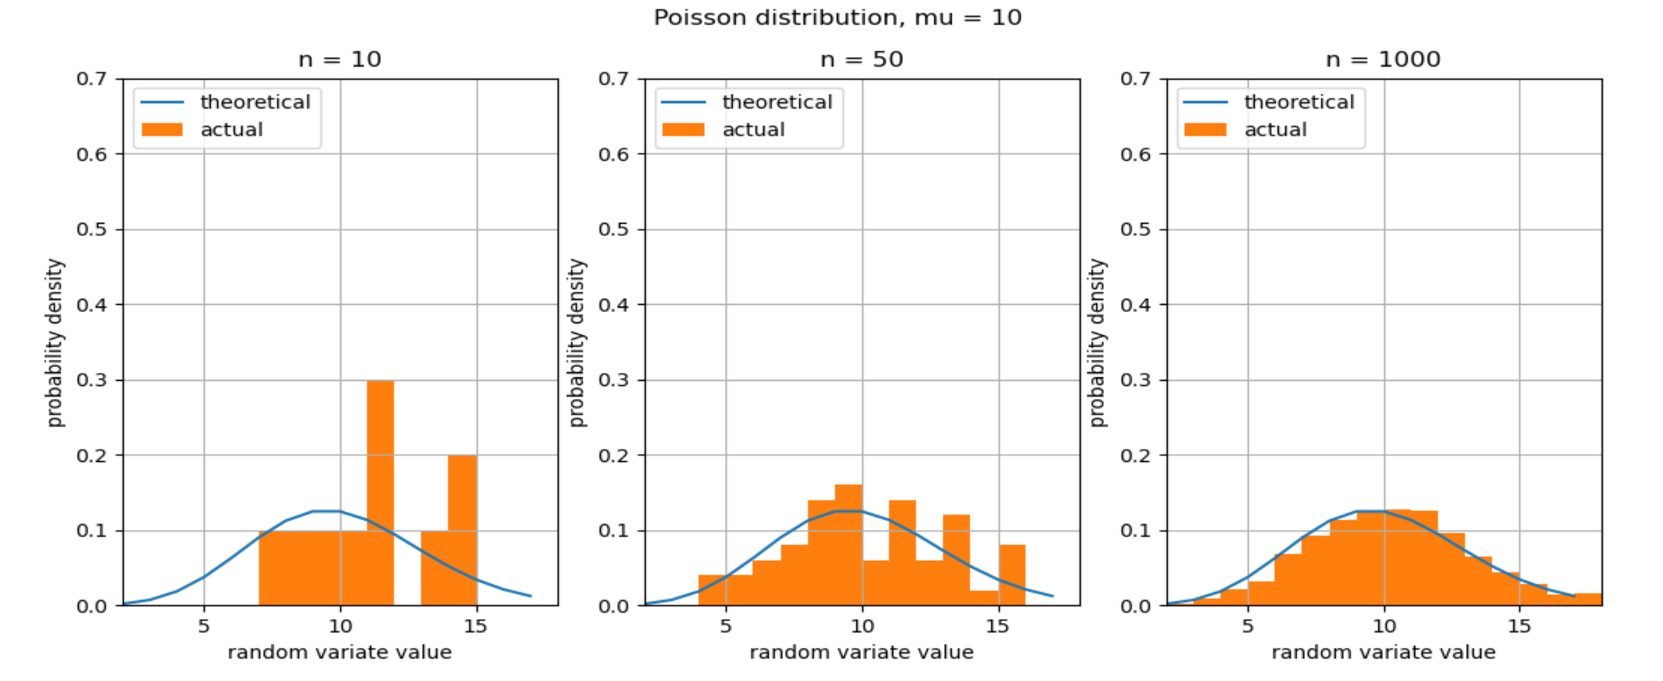
\includegraphics[width=\linewidth]{MS1res/poisson.png}
			\caption{Графики распределения Пуассона и сгенерированной выборки}
		\end{figure}
	\section{Обсуждение}
	Кратко описать полученные результаты можно следующим образом:\\
	На графиках с увеличением размеров выборки мы наблюдаем сходимость гистограмм к фигурам под графиками кривых распределения. Это объясняется тем, что данные гистограммы нормированны, т.е. суммарная площадь всех столбцов равна единице (как и площади под графиками каждой из кривой, что присуще функциям распределения вероятностей, ведь максимальное значение вероятности равно 1). Высота каждого столбца гистограммы прямо пропорциональна числу вхождений элементов случайной выборки в интервал, которому соответствует данный столбец (а в случае дискретного случая распределения Пуассона - числу соответствующих данному столбцу одинаковых целочисленных значений). Например, в случае распределения Коши для n = 10 все десять столбцов одинаковой высоты, что означает, что в каждый из этих интервалов попало ровно по одному элементу выборки. Благодаря нормированности гистограмм с увеличением выборки высоты столбцов распределяются соответствующим образом, а именно - число вхождений элементов выборки в интервалы все больше соответствует своему закону распределения.
	\section{Приложения}
	\noindent [1] Исходный код приложения на Python.\\ URL:{\url{https://github.com/via8/MathStat/tree/master/Lab1}}
\end{document}